% ex: ts=2 sw=2 sts=2 et filetype=tex
% SPDX-License-Identifier: CC-BY-SA-4.0

\documentclass[10pt,addpoints]{exam}

\usepackage[utf8]{inputenc}
\usepackage[T1]{fontenc}
%\usepackage[spanish]{babel}
\usepackage[letterpaper]{geometry}
\usepackage{graphicx}
\usepackage{pgfplots}
\usepackage{multicol}
\setlength{\columnsep}{2cm}

\pagestyle{headandfoot}
\headrule
\header{Matemáticas aplicadas}{Intersemestrales}{CBTIS 246}
\footer{}{Página \thepage\ de \numpages}{}

\pointpoints{punto}{puntos}
\renewcommand{\solutiontitle}{\textbf{Solución: }}

\printanswers

\begin{document}

Nombre:\enspace\hrulefill

\vspace{5mm}

Grupo:\enspace\hrulefill
\enspace{}Grado:\enspace\hrulefill
\enspace{}Fecha:\enspace\hrulefill

\begin{questions}

\begin{EnvFullwidth}
  \sffamily\textbf{Investiga y respesponde las siguientes pregutnas.}
\end{EnvFullwidth}

% ex: ts=2 sw=2 sts=2 et filetype=tex
% SPDX-License-Identifier: CC-BY-SA-4.0

\question ¿Qué es una sucesión o progreción?
  \begin{solution}[2cm]
    Es un conjunto de números ordenados que siguen un patrón o regla
    especifica.
  \end{solution}

% ex: ts=2 sw=2 sts=2 et filetype=tex
% SPDX-License-Identifier: CC-BY-SA-4.0

\question Una empresa exporta 10 toneladas de maiz y tiene una ganancia de
          \$25,000. ¿Cuánto será la ganancia si exporta 30 toneladas?

  \begin{solution}[2cm]
      $\frac{30 \times 25,000}{10} = 75,000$
  \end{solution}

% ex: ts=2 sw=2 sts=2 et filetype=tex
% SPDX-License-Identifier: CC-BY-SA-4.0

\question ¿Qué tipos de sucesiónes hay?:
  \begin{solution}[2cm]
    Se clasifican en aritméticas, gemétricas, alfanuméricas y simbólicas
  \end{solution}

% ex: ts=2 sw=2 sts=2 et filetype=tex
% SPDX-License-Identifier: CC-BY-SA-4.0

\question Sobre un cuerpo de $33$kg actua una fuerza de $297$\textbf{N}
          ¿Qué aceleración le proporciona dicha fuerza al cuerpo?

\makenonemptybox{1.6in}{Datos: \hspace{1cm} Formula: \hspace{1cm}
                      Despeje: \hspace{1cm} Sustitución y Resultado}

% ex: ts=2 sw=2 sts=2 et filetype=tex
% SPDX-License-Identifier: CC-BY-SA-4.0

\question Dos magnitudes son inversamente proporcionales cuando al aumentar
          una, la otra disminuye en la misma proporción. A esto se le llama:
          \fillin[Proporcional inversa]

% ex: ts=2 sw=2 sts=2 et filetype=tex
% SPDX-License-Identifier: CC-BY-SA-4.0

\question $x^2 - 9x + 8$



\newpage

% ex: ts=2 sw=2 sts=2 et filetype=tex
% SPDX-License-Identifier: CC-BY-SA-4.0

\question $c^2 + 5c - 24$


% ex: ts=2 sw=2 sts=2 et filetype=tex
% SPDX-License-Identifier: CC-BY-SA-4.0

\question ¿Qué es rotación, traslación y percepción espacial?:


%%%%%%%%%%%%%%%%%%%%%%%%%%%%%%%%%%%%%%%%%%%

\begin{EnvFullwidth}
  \sffamily\textbf{Une con una línea la respuesta que corresponde.}
\end{EnvFullwidth}

% ex: ts=2 sw=2 sts=2 et filetype=tex
% SPDX-License-Identifier: CC-BY-SA-4.0

\begin{multicols}{2}
  \question Son secuencias de números reales ordenados y deben tener un
            primer termino.

  \question Son las sucesiones donde el término siguiente se obtiene
            multiplicando al anterior por una cantidad constante llamada
            razón.

  \question Es la sucesión que consta de números y letras.

\columnbreak

  \begin{enumerate}
    \item[a)] Suseciones alfanumericas
    \vspace{\baselineskip}
    \item[b)] Sucesiones
    \vspace{\baselineskip}
    \item[c)] Sucesiones geométricas
    \vspace{\baselineskip}
    \item[d)] Secuencias numéricas
  \end{enumerate}
\end{multicols}


\begin{EnvFullwidth}
  \sffamily\textbf{Lee con atención cada pregunta y responde en
  el espacio indicado. }
\end{EnvFullwidth}

% ex: ts=2 sw=2 sts=2 et filetype=tex
% SPDX-License-Identifier: CC-BY-SA-4.0

\question De la siguiente suceción
\[
2,7,12,17
\]
\begin{parts}
  \part Escribe los 4 números siguientes: \fillin[22][1.5cm],
  \fillin[27][1.5cm], \fillin[32][1.5cm], \fillin[37][1.5cm].

  \part ¿Cuál es la diferencia? \fillin[5]

  \part Crea un modelo matemático que la represente: \fillin[2 + 5(n)]

  \part Calcula los términos de $n_3=$\fillin[17][1.5cm],
  $n_7=$\fillin[37][1.5cm], $n_9=$\fillin[47][1.5cm],
  $n_{25}=$\fillin[157][1.5cm].
\end{parts}

\vspace{\baselineskip}

% ex: ts=2 sw=2 sts=2 et filetype=tex
% SPDX-License-Identifier: CC-BY-SA-4.0

\question \[ \frac{7}{5} - \frac{5}{5} = \frac{\hspace{2cm}}{\hspace{2cm}}
             \hspace{2cm}
             \frac{2}{2} - \frac{1}{4} = \frac{\hspace{2cm}}{\hspace{2cm}}
          \]

\vspace{\baselineskip}

% ex: ts=2 sw=2 sts=2 et filetype=tex
% SPDX-License-Identifier: CC-BY-SA-4.0

\question $8xy(9x^3y - 6x^2y - 3xy^3) = $

  \begin{oneparchoices}
    \CorrectChoice $72x^4y^2 - 48x^3y^2 - 24x^2y^4$
    \choice $72x^4y^2 + 48x^3y^2 + 24x^2y^4$
    \choice $17x^4y^2 - 14x^3y^2 - 12x^2y^4$
    \choice $17x^4y^2 + 14x^3y^2 + 12x^2y^4$
  \end{oneparchoices}


\vspace{\baselineskip}

% ex: ts=2 sw=2 sts=2 et filetype=tex
% SPDX-License-Identifier: CC-BY-SA-4.0

\question Es solo una pequeña parte de la población:

  \begin{oneparchoices}
    \CorrectChoice Muestra
    \choice Individuo
    \choice Dato
  \end{oneparchoices}


%%%%%%%%%%%%%%%%%%%%%%%%%%%%%%%%%%%%%%%%%%%

\begin{EnvFullwidth}
  \sffamily\textbf{Selecciona la respuesta correcta. }
\end{EnvFullwidth}

\vspace{\baselineskip}
% ex: ts=2 sw=2 sts=2 et filetype=tex
% SPDX-License-Identifier: CC-BY-SA-4.0

\question $x^2 - 25$


\vspace{\baselineskip}
% ex: ts=2 sw=2 sts=2 et filetype=tex
% SPDX-License-Identifier: CC-BY-SA-4.0

\question $a^2 - 64$


% ex: ts=2 sw=2 sts=2 et filetype=tex
% SPDX-License-Identifier: CC-BY-SA-4.0

\question Una urna contiene canicas de colores: 8 Azules, 12 moradas,
4 negras y 16 rojas. Completa los siguientes espacios de la tabla y
determina cuál es la probabiliad de que al hacer una extracción esta
sea de color ... 

  \begin{tabular}{|l|c|c|l|l|l|}
    \hline
    \textbf{Evento} &  \textbf{Casos} & \textbf{Casos} &
    \textbf{Probabilidad} & \textbf{Decimal} &  \textbf{Porcentaje} \\
     &  \textbf{favorables} & \textbf{posibles} & & & \\
    \hline
    Azul & & & & & \\
    \hline
    Morado & & & & & \\
    \hline
    Negro & & & & & \\
    \hline
    Rojo & & & & & \\
    \hline
    \textbf{Suma} & & \textbf{Suma} & & & \\
    \hline
  \end{tabular}

% ex: ts=2 sw=2 sts=2 et filetype=tex
% SPDX-License-Identifier: CC-BY-SA-4.0

\question 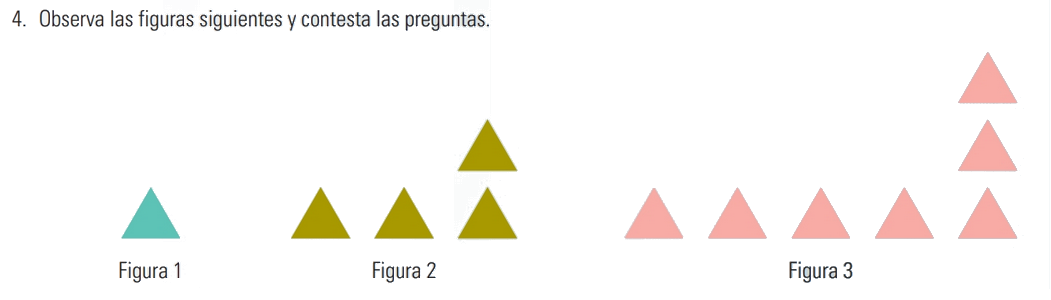
\includegraphics[scale=0.4]{p/i021.png} 
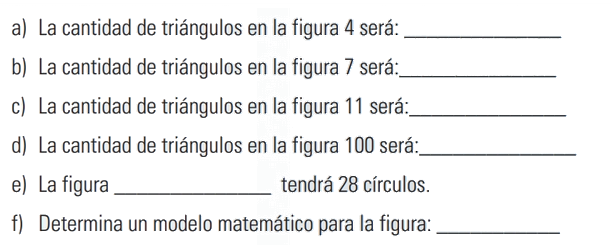
\includegraphics[scale=0.5]{p/i031.png} 

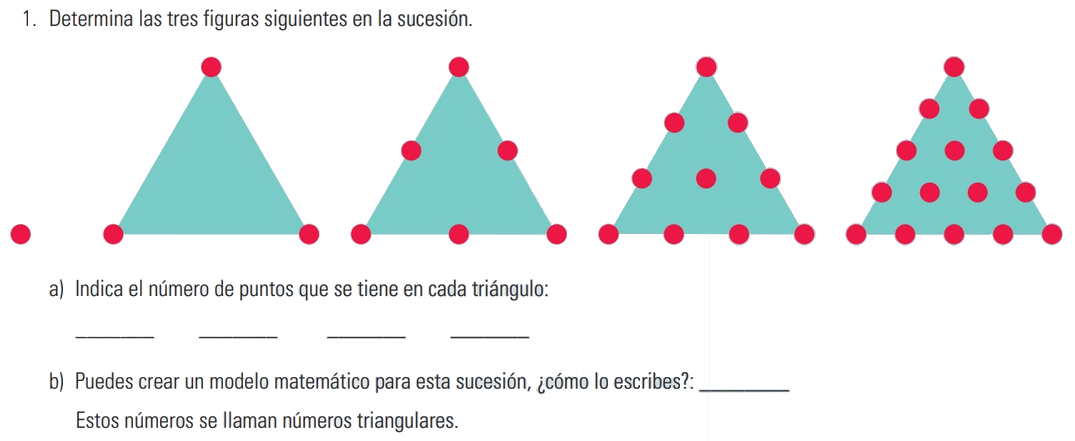
\includegraphics[scale=0.4]{p/i041.png} 
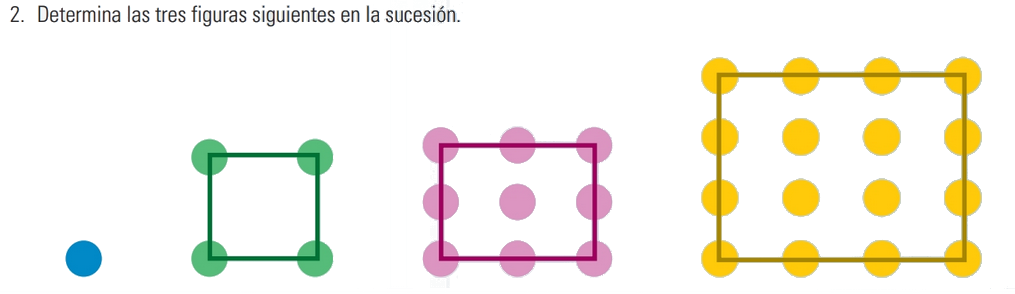
\includegraphics[scale=0.4]{p/i051.png} 


\includegraphics[scale=0.4]{p/i061.png} 


%%%%%%%%%%%%%%%%%%%%%%%%%%%%%%%%%%%%%%%%%%%

\newpage

% ex: ts=2 sw=2 sts=2 et filetype=tex
% SPDX-License-Identifier: CC-BY-SA-4.0

\question Una urna contiene canicas de colores: 10 son azules, 5 son
blancas, 12 son color café, 8 son doradas y 5 son color esmeralda. ¿Cuál es
la probabilidad de que al sacar una canica esta sea de color ...?

  \begin{tabular}{|l|c|c|l|l|l|}
    \hline
    \textbf{Evento} &  \textbf{Casos} & \textbf{Casos} &
    \textbf{Probabilidad} & \textbf{Decimal} &  \textbf{Porcentaje} \\
     &  \textbf{favorables} & \textbf{posibles} & & & \\
    \hline
    Azul & & & & & \\
    \hline
    Blanca & & & & & \\
    \hline
    Café & & & & & \\
    \hline
    Dorada & & & & & \\
    \hline
    Esmeralda & & & & & \\
    \hline
    \textbf{Suma} & & \textbf{Suma} & & & \\
    \hline
  \end{tabular}


\newpage

% ex: ts=2 sw=2 sts=2 et filetype=tex
% SPDX-License-Identifier: CC-BY-SA-4.0

\question $x^2 + 8x + 16$

% ex: ts=2 sw=2 sts=2 et filetype=tex
% SPDX-License-Identifier: CC-BY-SA-4.0

\question Resuelve las siguientes ecuaciones y compruebalos sustituyendo el
          valor de $x$

  \begin{parts}
    \part $6x+4 = 3x+10$ \\
    \\
    \\
    \\
    \part $6x+3 = 2x+11$ \\
    \\
    \\
    \\
    \part $2x+5 = x-3$
  \end{parts}


\end{questions}

\end{document}
